\documentclass[conference]{IEEEtran}
\IEEEoverridecommandlockouts
\usepackage{cite}
\usepackage{amsmath,amssymb,amsfonts}
\usepackage{graphicx}
\usepackage{textcomp}
\usepackage{xcolor}
\usepackage{booktabs}
\usepackage{multirow}
\usepackage{tikz}
\usetikzlibrary{arrows.meta,positioning}
\usepackage[hidelinks]{hyperref}
\raggedbottom

\begin{document}

\title{Evaluating and Preserving Laboratory Relationships in Synthetic Clinical Tables}

\author{\IEEEauthorblockN{Naren Medarametla}
\IEEEauthorblockA{\textit{School Of Computer Science and Engineering} \\
\textit{Vellore Institute of Technology}\\
Chennai, India \\
naren.medarametla2023@vitstudent.ac.in}
\and
\IEEEauthorblockN{Abishek K G}
\IEEEauthorblockA{\textit{School Of Computer Science and Engineering} \\
\textit{Vellore Institute of Technology}\\
Chennai, India \\
abishek.kg2023@vitstudent.ac.in}
\and
\IEEEauthorblockN{Roshan Parveen}
\IEEEauthorblockA{\textit{School Of Computer Science and Engineering} \\
\textit{Vellore Institute of Technology}\\
Chennai, India \\
roshan.parveen2023@vitstudent.ac.in}

\and
\IEEEauthorblockN{Parkavi K}
\IEEEauthorblockA{\textit{School Of Computer Science and Engineering} \\
\textit{Vellore Institute of Technology}\\
Chennai, India \\
parkavi.k@vit.ac.in}
}

\maketitle

\begin{abstract}
Synthetic clinical tables are judged by empirical evaluation, yet laboratory data are small, reported on fixed grids and linked by formulas that hold exactly or only up to rounding. We study how such tables should be evaluated and how their relationships should be preserved. In a prospectively specified study with two public populations and twelve generator variants, moving from an uncorrected to a corrected pipeline reversed 25\% to 34\% of generator pairs and changed the top-ranked generator in 18 of 20 training samples; a decomposition traced the training effect to an epoch cap that left small tables undertrained, not to validation-based checkpoint selection. We then formalize relation reparameterization, which replaces one participant of each supplied relation by a learned residual, and test it in a hypergraph-guided diffusion model on five NHANES datasets from four survey cycles. Formulas computed exactly from reported values were reproduced best by recomputing them. Approximate blood count formulas needed their residuals kept and sampled jointly: recomputation over-corrected them and independent residual noise broke their coupling, whereas joint resampling of real residuals and learned residual coding preserved it. The learned model reproduced the approximate relations most closely in every setting, by a small margin over the best control, and was the most realistic generator below a membership threshold in five of ten settings, all at 250 or 1,000 records; TabDiff or simple controls were as realistic or more elsewhere. Membership diagnostics are not privacy guarantees, and the contribution of the hypergraph was not isolated.
\end{abstract}

\begin{IEEEkeywords}
synthetic data, tabular data, diffusion models, laboratory data, evaluation methodology, membership inference
\end{IEEEkeywords}

\section{Introduction}

Synthetic data are increasingly proposed as a way to share clinical tables without exposing patients. Whether a synthetic table is faithful, useful and safe is decided almost entirely by empirical evaluation: classifier two-sample tests, distances between marginal and joint distributions, models trained on synthetic data and tested on real data, checks of clinical rules, and distance-based or attack-based privacy diagnostics. Clinical tables are typically small, their laboratory values are heavy-tailed and reported on fixed grids, some measurements are missing, and several variables are linked by formulas. Some formulas hold exactly at the reported precision, such as a globulin value computed from reported total protein and albumin; others hold only approximately, such as red cell indices that an analyzer computes from unrounded internal measurements. These properties interact with ordinary training and evaluation choices in ways that are easy to overlook.

This work began as the development of a constraint-guided diffusion model for medical tables. Ten development iterations produced mixed, partition-dependent conclusions, and an audit showed that most of them were produced by training and evaluation choices rather than by the models. We describe seven such pitfalls and quantify them in a controlled study. We then use the corrected protocol to develop and test a generator that reproduces laboratory relationships, and we report where it is better than published generators and simple controls and where it is not.

Our contributions are threefold. First, we catalogue seven training and evaluation pitfalls, quantify how much they change the ranking of generators on two public populations, and decompose the training correction into its components. Second, we formalize relation reparameterization with learned residuals, a conditioning-based reconstruction direction and re-derivation of exactly reported values, and we position it against rule-based reconstruction of dependent features. Third, on five NHANES panel-by-cycle datasets we compare it with five published generators and with post-processing controls that use the same knowledge of the relations, including textbook re-derivation and joint resampling of real residuals, and we identify which treatment each kind of relation needs and where a learned model adds to simple controls.

\section{Related Work}

Tabular data generators range from statistical copulas to generative adversarial networks and variational autoencoders, of which CTGAN and TVAE are the standard references \cite{xu2019ctgan}. Diffusion models \cite{ho2020ddpm,austin2021d3pm} were adapted to mixed tables by TabDDPM \cite{kotelnikov2023tabddpm}, which combines Gaussian and multinomial diffusion, and by TabDiff \cite{shi2025tabdiff}, which uses continuous-time diffusion with learnable per-column noise schedules. Feature relationships have been modeled with learned graphs in GOGGLE \cite{liu2023goggle}.

Umesh \textit{et al.} showed that common generators do not preserve functional dependencies between attributes \cite{umesh2024dependencies}, and their hierarchical feature generation framework generates independent features with an existing generator and reconstructs dependent features deterministically from supplied dependency rules \cite{umesh2025hfgf}. That framework targets mainly categorical dependencies and sets dependent values exactly by the rule. Our method differs in three respects: it models the discrepancy of each numerical relation as a learned residual instead of assuming exactness, it chooses which participant to reconstruct from the data to limit error propagation, and it accounts for the recording resolution of reported values. Constraint-aware generation also includes the constraint layers of C-DGM \cite{stoian2024cdgm} and DRL \cite{stoian2025drl} and the inference-time manifold guidance of Harpoon \cite{shankar2026harpoon}. We did not run these methods. Our deterministic re-derivation controls enforce the supplied relations exactly after generation and should not be read as reimplementations of them.

Evaluation commonly combines classifier two-sample tests \cite{lopezpaz2017c2st}, marginal and dependence distances, downstream utility and privacy diagnostics such as distance to the closest record, membership inference by overfitting detection \cite{vanbreugel2023domias} and attack-based audits \cite{giomi2023anonymeter}. The difficulty of estimating uncertainty from overlapping resamples is well known \cite{bengio2004variance}. We do not propose a new metric family; we show how ordinary choices around established metrics change conclusions on small clinical tables.

\section{The Seven Pitfalls}

The first pitfall is an under-specified training recipe for diffusion models on small tables. The legacy recipe of our case study stopped training by patience on a validation diffusion loss computed with one fixed draw of noise levels and masks, within a cap of 100 epochs. On a few hundred records this criterion is a noisy finite-sample estimate and is often flat early in training, and the cap itself allows only about 400 parameter updates at 200 training rows, against 5,000 in the corrected recipe, which also decays the learning rate and averages the weights. The symptom is a cluster of selected checkpoints near the start of training or at the cap. Section VI shows that the update budget, not the selection rule, accounts for most of the damage.

The second pitfall is linear scaling of heavy-tailed laboratory values. Standardization leaves most of the mass of an enzyme or triglyceride distribution in a tiny region while rare extreme values dominate the loss. A rank-based representation fitted on training rows, with a bounded inverse, is the usual alternative, but its benefit must be validated rather than assumed.

The third pitfall is ignoring the recorded measurement resolution. Laboratories report on fixed grids, sometimes depending on magnitude, as with significant-figure reporting of thyroid stimulating hormone. Continuous outputs fall off the grid and are detectable by tree-based discriminators, whereas resampling-based generators emit observed values and are implicitly favored. Every continuous-output generator should be decoded to the resolution detected on its training rows.

The fourth pitfall is scoring clinical rules by violation counts. For a relation computed exactly from reported values, the real violation rate is zero and recomputing the derived variable is correct practice. For an empirical envelope, such as a tolerance set at the 95th percentile of training residuals, about 5\% of real records violate the rule by construction, so zero violations signals over-correction. Rule behavior should be compared with real held-out behavior.

The fifth pitfall is training baselines outside their published recipes. Adapters that change optimization, for example by using a constant learning rate with early stopping, can make a strong method appear unstable. Baselines should reproduce the upstream training loop and document every adaptation.

The sixth pitfall is that realism metrics reward memorization. Copies of training records are indistinguishable from real data, so when generators or configurations are selected by two-sample tests, near-copying wins on small tables. Membership diagnostics should be reported beside every realism metric, and selection should respect a privacy threshold.

The seventh pitfall is the use of small evaluation sets. A two-sample AUROC estimated on tens to a hundred records per class is noisy, and generator orderings at that size often disagree with orderings on large reference sets. Evaluation should use the largest available held-out reference, with repeated subsampling and reported uncertainty.

\section{Case Study: A Development Project}

\begin{figure}[t]
\centering
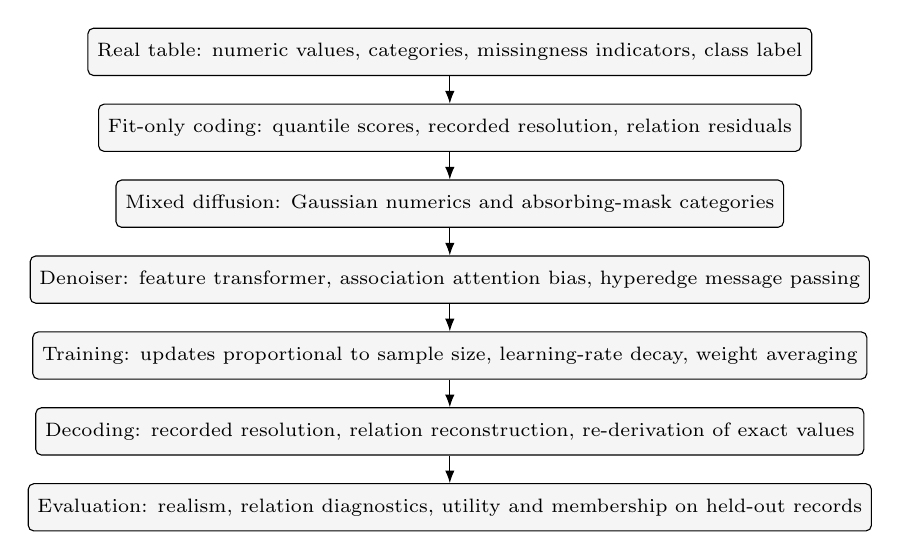
\begin{tikzpicture}[node distance=3.5mm, every node/.style={font=\scriptsize, align=center}, box/.style={draw, rounded corners=2pt, minimum width=7.6cm, minimum height=6mm, fill=gray!8}, arr/.style={-{Latex[length=1.6mm]}}]
\node[box] (a) {Real table: numeric values, categories, missingness indicators, class label};
\node[box, below=of a] (b) {Fit-only coding: quantile scores, recorded resolution, relation residuals};
\node[box, below=of b] (c) {Mixed diffusion: Gaussian numerics and absorbing-mask categories};
\node[box, below=of c] (d) {Denoiser: feature transformer, association attention bias, hyperedge message passing};
\node[box, below=of d] (e) {Training: updates proportional to sample size, learning-rate decay, weight averaging};
\node[box, below=of e] (f) {Decoding: recorded resolution, relation reconstruction, re-derivation of exact values};
\node[box, below=of f] (g) {Evaluation: realism, relation diagnostics, utility and membership on held-out records};
\foreach \x/\y in {a/b,b/c,c/d,d/e,e/f,f/g} \draw[arr] (\x) -- (\y);
\end{tikzpicture}
\caption{Overview of the corrected MedHyperDiff pipeline and its evaluation.}
\label{fig:pipeline}
\end{figure}

MedHyperDiff is a mixed-type diffusion model with Gaussian diffusion for numerical values, absorbing-mask diffusion for categories and explicit missingness indicators (Fig.~\ref{fig:pipeline}). Its denoiser is a feature transformer with an attention bias from a bootstrap-stable association graph and nonlinear hyperedge message passing over supplied clinical relations. Ten development iterations on four public UCI cohorts (Indian Liver Patient Dataset, heart failure, chronic kidney disease and early-stage diabetes) had produced partition-dependent effects and a repaired Gaussian copula that dominated the model on realism and rule compliance.

The audit found that 13 of 36 fits in one iteration stopped during the initial plateau of the validation loss and kept checkpoints from epochs 3 to 28, while the other 23 reached the 100-epoch cap still improving. Enzyme and bilirubin values were linearly scaled, every numerical column had a fixed reporting grid but outputs were continuous, an empirical protein tolerance was scored as if fewer violations were always better, and the TabDDPM adapter used a constant learning rate with early stopping instead of the upstream recipe. The modified implementation reproduces an archived synthetic table byte for byte under the original settings, so each correction can be isolated.

Table~\ref{tab:ablation} and Fig.~\ref{fig:ablation} apply the corrections one at a time on three development partitions of the liver dataset with three seeds each. The training correction alone reduced association error by 61\%, to the level of a control that resamples training rows, and restoring only the original training loop, with its epoch cap and validation-selected checkpoint, undid most of that gain. Decoding to the recorded resolution produced most of the remaining improvement in two-sample realism, measured as the AUROC of a classifier separating synthetic from real records (C2ST), where 0.5 means indistinguishable.

\begin{table}[t]
\caption{Correcting one pitfall at a time (liver dataset, development partitions)}
\label{tab:ablation}
\centering
\setlength{\tabcolsep}{4pt}
\begin{tabular}{lcccc}
\toprule
Variant & C2ST & Num. W & Assoc. & Rule gap \\
\midrule
Original recipe & 0.855 & 0.245 & 0.176 & 0.004 \\
+ corrected training recipe & 0.730 & 0.167 & 0.068 & 0.006 \\
+ quantile coding, 100 steps & 0.714 & 0.151 & 0.066 & 0.006 \\
+ recorded resolution & \textbf{0.571} & \textbf{0.150} & \textbf{0.066} & \textbf{0.001} \\
Corrected, original training loop & 0.697 & 0.166 & 0.158 & 0.002 \\
Repaired copula & 0.573 & 0.153 & 0.079 & 0.006 \\
Bootstrap copy control & 0.493 & 0.150 & 0.066 & 0.002 \\
\bottomrule
\end{tabular}
\end{table}

\begin{figure*}[t]
\centering
\includegraphics[width=\textwidth]{figures/fig_ablation.png}
\caption{Effect of each correction on the liver dataset development partitions (mean and standard deviation across three partitions). C2ST is the two-sample classifier AUROC (0.5 is indistinguishable), numeric W the Wasserstein distance scaled by the training standard deviation, and the rule gap the difference between synthetic and real violation rates.}
\label{fig:ablation}
\end{figure*}

After correction, a comparison specified in advance with equal tuning budgets against upstream-recipe TabDDPM and TabDiff, CTGAN, TVAE and statistical references was evaluated once on reserved test folds. The corrected model improved on the original recipe in every seed and cohort, reducing C2ST from 0.944 to 0.631 on the liver data, from 0.761 to 0.615 on heart failure and from 0.782 to 0.586 on kidney disease. TabDiff and the copula were nevertheless more realistic overall. This stage also revealed the last two pitfalls: several TabDDPM configurations chosen by a fidelity and utility rule had membership AUROC between 0.91 and 0.99, and with 60 to 117 test patients the seed-to-seed standard deviation of C2ST reached 0.07.

\section{Controlled Study Design}

The case study cannot separate the pitfalls from one model's idiosyncrasies or from the noise of small test folds. The controlled study was specified in a dated protocol before any generator was fitted to its data. It uses NHANES 2017 to 2018 \cite{nhanes} adults with a standard biochemistry record (4,756 records, diagnosed diabetes as label, 21 numerical predictors and sex), in which globulin equals total protein minus albumin and body mass index equals weight over squared height as reported, and the UCI thyroid registry (9,172 records, any thyroid diagnosis as label, six numerical and sixteen categorical predictors, up to 28\% missing), in which the free thyroxine index approximately equals total thyroxine divided by thyroid hormone uptake.

Each population is split once into a reference half and a pool, grouped by identical predictor profile and stratified by label. From the pool, samples of nominal size $n = 250$ and $n = 1{,}000$ are drawn five times each and split 80/20 into 200 or 800 fit rows and validation rows. All generators fit the same rows, and every generator produces five synthetic records per fit row. The reference half, with 2,378 and 4,588 records, is never fitted and serves for utility, two-sample tests and as the source of non-members and attacker background data. Twelve variants are compared: corrected MedHyperDiff, the same with the legacy training recipe or linear scaling, TabDDPM with the upstream recipe and with an earlier adapter loop, TabDiff, CTGAN, TVAE, a Gaussian copula, a copula with re-derivation of supplied relations, independent marginals, and bootstrap resampling as a copy control. Configurations are fixed in advance.

Every continuous-output generator emits raw values that are decoded after sampling in three ways using fit rows only: raw, a single global grid per column, and a magnitude-banded grid. We compute C2ST with a random forest discriminator on the full reference and at 50 to 1,000 records per source with ten subsamples each, numerical and dependence distances, forest utility trained on synthetic and tested on real data (TSTR), rule violation rates and rule realism, a nearest-distance membership attack and a density-ratio membership attack in the style of DOMIAS \cite{vanbreugel2023domias}. Rankings are compared by the fraction of generator pairs whose order reverses and by Kendall's $\tau$, with bootstrap intervals over the five training samples.

\section{Results of the Controlled Study}

\subsection*{Uncorrected Versus Corrected Pipelines}

We ranked eight generator identities by realism under an uncorrected pipeline, consisting of diffusion models trained with the legacy recipe, the adapter TabDDPM loop, raw outputs, two-sample tests on 100 records per source and no privacy check, and under the corrected pipeline. The uncorrected pipeline combines the choices of our development project; we make no claim about how often these choices occur in published work. Table~\ref{tab:pipeline} and Fig.~\ref{fig:pipeline_rev} show that a quarter to a third of all pairwise comparisons reversed and that the top-ranked generator changed in 18 of 20 training samples. The case-study model ranked fourth to sixth of eight under the uncorrected pipeline in most samples and first in 16 of 20 under the corrected pipeline. With a privacy-aware ranking, which places generators with membership AUROC above 0.60 last, 20\% to 36\% of pairs reversed, and the corrected top generator was MedHyperDiff in three settings and the copula with re-derivation on thyroid at $n = 250$.

\begin{table}[t]
\caption{Agreement between uncorrected and corrected pipelines (realism ranking)}
\label{tab:pipeline}
\centering
\setlength{\tabcolsep}{3pt}
\begin{tabular}{lcccc}
\toprule
Population, $n$ & Pairs reversed & $\tau$ & Top-1 agree & Top (corrected) \\
\midrule
NHANES, 250 & 32\% (29 to 35) & 0.36 & 0/5 & MedHyperDiff \\
NHANES, 1,000 & 34\% (29 to 38) & 0.33 & 0/5 & MedHyperDiff \\
Thyroid, 250 & 25\% (22 to 28) & 0.50 & 0/5 & MedHyperDiff \\
Thyroid, 1,000 & 26\% (22 to 31) & 0.47 & 2/5 & MedHyperDiff \\
\bottomrule
\end{tabular}
\end{table}

\begin{figure*}[t]
\centering
\includegraphics[width=\textwidth]{figures/pipeline_reversals.png}
\caption{Fraction of generator pairs whose order reverses between uncorrected and corrected pipelines, for realism, privacy-aware realism and rule scoring (mean and 95\% bootstrap interval over five training samples).}
\label{fig:pipeline_rev}
\end{figure*}

\subsection*{Training Choices}

With the legacy recipe, 30\% of MedHyperDiff fits kept a checkpoint from the first 20 epochs, the earliest at epoch 3, and 45\% stopped at the cap. Its C2ST was worse than with the corrected recipe in all 20 paired samples, by 0.22 and 0.16 on NHANES and thyroid at $n = 250$ and by 0.17 and 0.07 at $n = 1{,}000$, and association error was also worse in all 20. A follow-up experiment, specified before it was run, decomposed this difference on the same samples (Table~\ref{tab:decomp}). Giving the corrected recipe only the legacy number of updates, 400 at 200 fit rows and 1,300 at 800, reproduced or exceeded the whole gap, with C2ST worse in all 20 samples by 0.17 on average. Returning the checkpoint with the lowest validation loss along the same trajectory instead of the final weights changed C2ST by 0.004 on average with no consistent sign, and so did averaging the validation loss over 16 corruption draws or stopping by patience. A constant learning rate without weight averaging did not consistently change realism but raised membership AUROC in all 20 samples, by 0.035 on average, while the undertrained variants had membership AUROC about 0.04 lower, in line with the trade-off between realism and memorization reported below. Rebuilding the legacy recipe inside the fixed-budget loop reproduced the legacy results. The first pitfall is therefore mainly an update budget set in epochs that is too small for small tables, not validation-based selection itself.

\begin{table}[t]
\caption{Decomposition of the training correction on the controlled-study samples (C2ST, mean of five samples; last column: samples of 20 in which C2ST was worse or better than with the corrected recipe)}
\label{tab:decomp}
\centering
\setlength{\tabcolsep}{2.4pt}
\begin{tabular}{lccccc}
\toprule
& \multicolumn{2}{c}{NHANES} & \multicolumn{2}{c}{Thyroid} & \\
Variant & 250 & 1,000 & 250 & 1,000 & Worse/better \\
\midrule
Corrected recipe & 0.729 & 0.691 & 0.710 & 0.686 & reference \\
+ validation-selected weights & 0.735 & 0.691 & 0.719 & 0.685 & 6/3 \\
+ selection with patience 20 & 0.778 & 0.691 & 0.710 & 0.685 & 5/6 \\
+ 16 corruption draws & 0.722 & 0.691 & 0.712 & 0.686 & 4/6 \\
Constant rate, raw weights & 0.786 & 0.689 & 0.754 & 0.683 & 13/7 \\
Legacy number of updates & 0.943 & 0.896 & 0.851 & 0.798 & 20/0 \\
Legacy, rebuilt & 0.945 & 0.832 & 0.862 & 0.760 & 20/0 \\
Legacy recipe & 0.951 & 0.857 & 0.866 & 0.756 & 20/0 \\
\bottomrule
\end{tabular}
\end{table}

The earlier TabDDPM adapter loop on the upstream architecture diverged, with C2ST between 0.995 and 1.000 and utility between 0.49 and 0.70, against 0.74 to 0.91 and 0.87 to 0.94 with the upstream recipe. Quantile coding lowered C2ST relative to linear scaling in three of four settings, by 0.02 to 0.07 in every sample, but raised it by 0.03 for NHANES at $n = 250$, so the representation is a choice to validate rather than a fixed rule.

\subsection*{Recording Resolution}

Decoding changed some generators by up to 0.31 and others not at all (Table~\ref{tab:precision}, Fig.~\ref{fig:precision}). The difference lies in the inverse transforms rather than the models. TabDDPM and TabDiff invert quantile transforms whose tied knots return 45\% to 98\% of values exactly on the recording grid, which acts as an implicit decoding, whereas MedHyperDiff, TVAE and CTGAN emit almost no on-grid values. Without explicit decoding, realism rankings reversed for 29\% to 32\% of generator pairs on NHANES and 7\% to 14\% on thyroid, and the top generator changed. On the thyroid data, where hormone values are reported to about two significant figures, a single grid per column recovered only part of the effect.

\begin{table}[t]
\caption{C2ST by decoding (nominal $n = 1{,}000$)}
\label{tab:precision}
\centering
\setlength{\tabcolsep}{3pt}
\begin{tabular}{lccccc}
\toprule
& \multicolumn{2}{c}{NHANES} & \multicolumn{3}{c}{Thyroid} \\
Generator & Raw & Decoded & Raw & Global & Banded \\
\midrule
MedHyperDiff & 0.999 & 0.692 & 0.808 & 0.763 & 0.685 \\
TVAE & 0.991 & 0.913 & 0.950 & 0.947 & 0.934 \\
TabDiff & 0.703 & 0.703 & 0.698 & 0.696 & 0.692 \\
TabDDPM & 0.744 & 0.738 & 0.742 & 0.747 & 0.745 \\
\bottomrule
\end{tabular}
\end{table}

\begin{figure*}[t]
\centering
\includegraphics[width=\textwidth]{figures/p3_precision_c2st.png}
\caption{C2ST against the reference population for raw outputs and outputs decoded to the recorded resolution (mean of five training samples).}
\label{fig:precision}
\end{figure*}

\subsection*{Rules and Memorization}

No learned generator reproduced the supplied relations. Between 90\% and 100\% of their NHANES records violated the globulin or body mass index identities at recorded resolution, against 0\% in real data, and most thyroid records violated the free thyroxine envelope, against about 5\% in real data. Re-deriving these variables from their operands reproduced real behavior. Scoring by violation counts rather than by the gap to real rates reversed 11\% to 22\% of generator pairs but not the winner.

Across generators, lower C2ST went with higher membership AUROC, with Spearman correlations between $-0.33$ and $-0.77$ (Fig.~\ref{fig:memo}). Excluding the copy control, the most realistic generator in a training sample exceeded a membership AUROC of 0.60 on at least one attack in 40\%, 0\%, 80\% and 20\% of samples for NHANES at $n = 250$ and $1{,}000$ and thyroid at $n = 250$ and $1{,}000$. Upstream TabDDPM reached 0.85 to 0.89 at $n = 250$. In the case-study search over 160 configurations, the most realistic configuration of a method exceeded the membership threshold in 10 of 20 cohort and method combinations.

\begin{figure*}[t]
\centering
\includegraphics[width=\textwidth]{figures/p6_memorization.png}
\caption{Realism against membership risk for each generator (mean of five training samples). Points above the dashed line exceed a membership AUROC of 0.60 on at least one of two attacks.}
\label{fig:memo}
\end{figure*}

\subsection*{Evaluation Size}

Table~\ref{tab:evalsize} and Fig.~\ref{fig:evalsize} report the probability that a single two-sample test orders a generator pair as the full reference does. At the 60 to 120 test patients typical of public clinical cohorts, about one comparison in six was ordered wrongly, and close competitors were separated little better than by chance. Agreement reached 90\% at about 500 records per source. These values are empirical for this discriminator and these populations rather than general sample-size requirements.

\begin{table}[t]
\caption{Probability that one evaluation orders a pair correctly}
\label{tab:evalsize}
\centering
\setlength{\tabcolsep}{4pt}
\begin{tabular}{lccccc}
\toprule
Records per source & 50 & 100 & 200 & 500 & 1,000 \\
\midrule
NHANES & 0.77 & 0.85 & 0.88 & 0.93 & 0.96 \\
Thyroid & 0.78 & 0.84 & 0.90 & 0.94 & 0.95 \\
Pairs differing by at most 0.02 & 0.58 & 0.59 & 0.58 & 0.65 & 0.71 \\
Median single-draw SD & 0.062 & 0.045 & 0.031 & 0.015 & 0.008 \\
\bottomrule
\end{tabular}
\end{table}

\begin{figure}[t]
\centering
\includegraphics[width=\columnwidth]{figures/p7_evaluation_size.png}
\caption{Agreement between a single two-sample test and the full reference ordering as a function of evaluation size. The dashed line marks 90\%.}
\label{fig:evalsize}
\end{figure}

\section{Relation Reparameterization}

\subsection*{Relations and Residuals}

A supplied relation $k$ links a derived variable $x_{d_k}$ to operands $x_{O_k}$ through a known function, $x_{d_k} = f_k(x_{O_k}) + \varepsilon_k$, where $\varepsilon_k$ collects rounding and analyzer effects and is zero only for relations computed exactly. Every participant $j \in P_k = \{d_k\} \cup O_k$ can be solved for, $x_j = g_{kj}(x_{P_k \setminus j}) + \varepsilon_{kj}$. Relation reparameterization chooses one target $t_k \in P_k$ per relation and replaces $x_{t_k}$ by the residual
\begin{equation}
r_k = x_{t_k} - g_{k t_k}\!\left(x_{P_k \setminus t_k}\right).
\label{eq:residual}
\end{equation}
The generator models the joint distribution of the remaining variables and the residuals, so rounding noise and rare discrepancies are learned rather than forced to zero or ignored. After sampling, every generated variable is decoded to its recording resolution $\rho_j$, detected on fit rows, and the targets are reconstructed in an acyclic order,
\begin{equation}
\hat{x}_{t_k} = \rho_{t_k}\!\left( g_{k t_k}(\hat{x}_{P_k \setminus t_k}) + \hat{r}_k \right).
\label{eq:decode}
\end{equation}
A relation is treated as reported exactly when at least 99\% of complete fit rows satisfy $|x_{d_k} - f_k(x_{O_k})| \le \delta_{d_k}/2$, where $\delta_{d_k}$ is the recording step of the derived variable. For such relations the decoder finally sets $\hat{x}_{d_k} = \rho_{d_k}(f_k(\hat{x}_{O_k}))$, the computation the laboratory performs, so that rounding a reconstructed operand does not create discrepancies that real records do not have.

\subsection*{Choosing the Reconstructed Participant}

Errors in the generated participants propagate into the reconstructed one. On the scale on which relation $k$ is additive, $\sum_{j \in P_k} a_{kj}\, \phi_k(x_j) = c_k$, with $\phi_k$ the logarithm for products and ratios and the identity for sums, differences and linear formulas, a generation error $e_j$ in participant $j$ moves the reconstructed target $t$ by approximately $-a_{kt}^{-1} \sum_{j \ne t} a_{kj} e_j$. Relative to the spread of the target, $s_{kt} = |a_{kt}|\, \mathrm{sd}(\phi_k(x_t))$, this error is smallest for the participant with the largest $s_{kt}$ when generated participants have comparable errors. For body mass index, which is additive on the logarithmic scale as $\log \mathrm{BMI} = \log w - 2\log h + c$, height therefore enters with coefficient 2. We therefore choose
\begin{equation}
(t_1, \dots, t_K) = \arg\max \textstyle\sum_{k} s_{k t_k}
\label{eq:choice}
\end{equation}
over assignments with distinct targets that admit an acyclic reconstruction order, estimating $s$ on fit rows only. The rule rests on this first-order argument and is a heuristic, not a guarantee of optimal conditioning. It enumerates $\prod_k |P_k|$ assignments, 135 for the four blood count relations used below, which is small for a laboratory panel but grows exponentially with the number of relations.

\subsection*{Model, Training and Evaluation of Relations}

In MedHyperDiff each residual and the participants it depends on, expanded recursively through earlier reconstructions, form a hyperedge of the denoiser. The model is trained with a velocity-prediction loss on observed numerical values, an absorbing-state cross-entropy for categories and observation indicators, and a small physical-range energy, with linear learning-rate decay and weight averaging. The number of updates is $5{,}000 \max(1, n/250)$ for nominal sample size $n$, so the number of passes over the fit rows is constant. Table~\ref{tab:config} lists the complete configuration.

\begin{table}[t]
\caption{Final MedHyperDiff configuration}
\label{tab:config}
\centering
\setlength{\tabcolsep}{3pt}
\begin{tabular}{p{1.9cm}p{6.1cm}}
\toprule
Component & Setting \\
\midrule
Coding & Fit-only normal-quantile scores with bounded inverse for numerical values; categories and one observation indicator per numerical variable as categorical tokens; one residual per supplied relation \\
Diffusion & 100 steps; cosine schedule and velocity prediction for numerical values; absorbing-mask diffusion for categorical tokens \\
Denoiser & Width 32; two blocks, each a hypergraph block followed by four-head self-attention with an additive bias from the association graph and a feed-forward layer; time and class-label embeddings \\
Association graph & Spearman magnitude for numerical pairs, binned normalized mutual information otherwise; an edge is kept if its value is at least 0.15 on the fit rows and in at least 60\% of 10 bootstrap resamples \\
Hyperedges & Each residual with the participants it depends on, expanded through earlier reconstructions \\
Loss & Velocity error on observed numerical values, $T/t$-weighted cross-entropy on masked tokens, physical-range energy with weight 0.01 \\
Optimization & AdamW, learning rate $10^{-3}$ decayed linearly to zero, weight decay $10^{-4}$, batch 64, gradient clipping at 1, $5{,}000\max(1, n/250)$ updates, weight averaging with decay 0.999, final averaged weights; observation heads initialized at fit frequencies \\
Sampling & 100 reverse steps conditioned on the class labels of the fit rows, five records per fit row, no guidance; decoding to the recorded resolution, reconstruction and re-derivation \\
\bottomrule
\end{tabular}
\end{table}

We score relation $k$ by
\begin{equation}
D_k = W_1\!\left(|\hat{\varepsilon}_k|, |\varepsilon_k^{\mathrm{ref}}|\right) / \max\!\left(\sigma_k, \delta_{d_k}/\sqrt{48}\right),
\label{eq:metric}
\end{equation}
the Wasserstein distance between absolute residuals of synthetic and held-out reference records, scaled by $\sigma_k$, the standard deviation of absolute residuals on fit rows, floored at the value for pure rounding. The relation distance is the mean of $D_k$ over relations. Because absolute residuals discard the sign of a discrepancy and its dependence on other variables, we also report signed distances, the agreement of Spearman correlations between each residual and its participants, age and the label, the agreement of correlations between residuals of different relations, tail exceedance and coverage.

\section{A First Test on Blood Counts}

The method was first tested on the complete blood count panel of NHANES 2017 to 2018 (4,865 adults). The panel had not been used before, but 4,753 of its participants also belong to the biochemistry population of the controlled study. The analyzer measures red cell count, hemoglobin and mean corpuscular volume and computes hematocrit, mean corpuscular hemoglobin and mean corpuscular hemoglobin concentration, and the five white cell differential percentages sum to 100, all up to rounding of unrounded internal values. During development, reconstructing the basophil fraction or the mean corpuscular hemoglobin concentration, which are narrow quantities, raised C2ST to between 0.84 and 0.88; the rule of Eq.~(\ref{eq:choice}) instead reconstructs red cell count, hemoglobin, mean corpuscular hemoglobin and the neutrophil percentage. The variant was chosen on a separate development pool with a rule fixed in advance and evaluated on a never-fitted reference half of 2,433 records with five samples per size. Published generators were compared as generated and with post-processings of the same output that use the same knowledge of the relations: deterministic re-derivation in the reconstruction direction of our rule or in the textbook direction, and derivation plus real residuals, resampled independently for each relation or jointly as the complete residual vector of one real record. The textbook and joint variants were added after the confirmation, as described in Section IX. The same reparameterization was also applied to TabDiff.

\begin{table}[t]
\caption{Blood count 2017 to 2018 (mean of five samples). Best other arm: lowest relation distance among all comparator arms, or lowest C2ST and highest TSTR AUROC among comparator arms with membership AUROC at most 0.60: $^{a}$TVAE with joint residuals, $^{b}$copula with rule-direction re-derivation, $^{c}$copula with independent residuals, $^{d}$TabDiff with rule-direction re-derivation, $^{e}$TabDiff with reparameterization. Wins: samples in which MedHyperDiff was better than that arm}
\label{tab:relation}
\centering
\setlength{\tabcolsep}{3pt}
\begin{tabular}{llcccc}
\toprule
$n$ & Measure & Ours & TabDiff & Best other arm & Wins \\
\midrule
\multirow{4}{*}{250} & Relation dist. & \textbf{0.187} & 12.14 & 0.199$^{a}$ & 3/5 \\
& C2ST & \textbf{0.691} & 0.762 & 0.731$^{b}$ & 5/5 \\
& TSTR AUROC & \textbf{0.717} & 0.670 & 0.687$^{c}$ & 5/5 \\
& Membership & 0.555 & 0.619 & 0.528$^{b}$ & \\
\midrule
\multirow{4}{*}{1,000} & Relation dist. & \textbf{0.173} & 3.92 & 0.176$^{a}$ & 2/5 \\
& C2ST & 0.664 & 0.645 & \textbf{0.633}$^{d}$ & 0/5 \\
& TSTR AUROC & 0.735 & 0.735 & \textbf{0.742}$^{e}$ & 1/5 \\
& Membership & 0.509 & 0.560 & 0.561$^{d}$ & \\
\bottomrule
\end{tabular}
\end{table}

\begin{figure*}[t]
\centering
\includegraphics[width=\textwidth]{figures/relation_fidelity_final.png}
\caption{Reproduction of the four blood count relations on the 2017 to 2018 reference half (mean of five samples, logarithmic scale). Blue: MedHyperDiff with relation reparameterization; green: published generators with joint residual resampling.}
\label{fig:relation}
\end{figure*}

Table~\ref{tab:relation} and Fig.~\ref{fig:relation} summarize the result. With $n = 250$ the model reproduced the four relations more closely than every published generator as generated, with relation distances of 12 to 244, or re-derived in either direction, with distances of 0.95 to 1.11, in all five samples, and more closely than every residual-resampling control in at least three of five samples; the closest control, TVAE with joint residuals, reached 0.199 against 0.187. It also had a lower C2ST than every comparator arm with membership AUROC at most 0.60, 0.691 against 0.731, and higher utility, 0.717 against 0.687, with a membership AUROC of 0.555. With $n = 1{,}000$ it remained closer than the generators as generated or re-derived in every sample, but joint residual resampling was nearly as close, 0.176 against 0.173 with two wins in five samples, and TabDiff with re-derivation was more realistic, with a C2ST of 0.633 against 0.664. This model used 5,000 updates at every sample size, which the next section shows to be the cause of the latter.

\section{Robustness Across Survey Cycles, Relation Types and Sizes}

\subsection*{Design}

A second study, again specified in a dated protocol before fitting, asked whether the relation result replicates in other survey cycles, whether it extends to relations of another kind, how it changes with sample size, and whether reparameterization also helps other generators. Four confirmation datasets were built from NHANES public files: blood counts from 2013 to 2014 (5,229 adults) and 2021 to 2023 (5,555), and a chemistry panel from 2011 to 2012 (4,778) and 2021 to 2023 (5,284). The chemistry panel has 20 numerical variables from anthropometry, the standard biochemistry profile and urine tests, with four relations that NHANES computes from reported values: globulin as total protein minus albumin, body mass index, the urine albumin to creatinine ratio, and calculated serum osmolality, $1.86\,\mathrm{Na} + \mathrm{glucose}/18 + \mathrm{BUN}/2.8 + 9$. An audit before fitting found every chemistry relation exact at reported precision and no blood count relation exact. These datasets are panel-by-cycle datasets rather than independent populations. NHANES samples different people in each cycle, but the two 2021 to 2023 datasets share 5,263 participants, and the two development datasets from 2015 to 2016, used only to choose the training budget, share 5,019. The blood count results therefore come from three survey cycles and the chemistry results from two.

Each dataset was split once into a never-fitted reference half and a pool. Samples of nominal size 250 and 1,000 (200 and 800 fit rows) were drawn five times, and samples of 2,000 (1,600 fit rows) three times in the two 2021 to 2023 datasets. Two replicate samples share about 30\% of their fit rows at $n = 1{,}000$ and about 60\% at $n = 2{,}000$, so the spread over replicates understates sampling variability, and all differences below are conditional on the fixed reference halves. The published generators kept their fixed configurations, whereas the training budget of our model was chosen on the development datasets among four candidates declared in advance: on development data, updates proportional to $n$ lowered the mean C2ST from 0.690 to 0.653, while wider networks did not help and raised membership AUROC. Published generators were evaluated as generated, with deterministic re-derivation in the reconstruction direction of our rule, with derivation plus independently resampled residuals, and fitted with reparameterization added. After the run and two external reviews we added two controls that use only saved outputs and the same knowledge of the relations: re-derivation of every derived variable in its textbook direction, which corresponds to rule-based reconstruction, and joint residual resampling, which gives each synthetic row the complete residual vector of one randomly drawn fit row with every residual observed and leaves a residual missing where the synthetic row lacks its participants. Both were evaluated with the full metric set. Every arm, including our model, counts as eligible for privacy-constrained comparisons only if its mean membership AUROC is at most 0.60. The protocol stated success criteria as win counts and point-estimate margins; these are descriptive criteria rather than significance tests, and the comparisons that include the added controls are exploratory. A size of 100 records was removed during the run by a recorded amendment, before any comparator output was examined. We analyzed 598 confirmation fits, 10 further fits on the 2017 to 2018 blood counts, 20 MedHyperDiff fits at $n = 100$ that had finished before the amendment and are reported separately because they have no comparators, and 560 evaluations of the added controls on saved outputs of both relation studies.

\begin{table*}[t]
\caption{Confirmation on four datasets (mean over samples; nominal $n$). Relation control: lowest relation distance among all comparator arms, that is published generators as generated, re-derived in either direction, with independently or jointly resampled residuals, or with reparameterization, chosen per setting in hindsight. Realism and utility comparators: the arm with the lowest C2ST or highest TSTR AUROC among comparator arms with mean membership AUROC at most 0.60. $\dagger$: MedHyperDiff exceeds that membership threshold. Bold: better value among eligible arms. Wins: samples in which MedHyperDiff was better}
\label{tab:robust}
\centering
\setlength{\tabcolsep}{4pt}
\begin{tabular}{llccccccccc}
\toprule
& & \multicolumn{3}{c}{Relation distance} & \multicolumn{3}{c}{C2ST} & \multicolumn{3}{c}{TSTR AUROC} \\
Dataset & $n$ & Ours & Control & Wins & Ours & Comparator & Wins & Ours & Comparator & Wins \\
\midrule
Blood count 2013-14 & 250 & \textbf{0.128} & 0.139 & 4/5 & \textbf{0.709} & 0.728 & 4/5 & \textbf{0.709} & 0.698 & 5/5 \\
 & 1,000 & \textbf{0.092} & 0.106 & 5/5 & 0.646 & \textbf{0.634} & 1/5 & \textbf{0.771} & 0.753 & 5/5 \\
Blood count 2021-23 & 250 & \textbf{0.151} & 0.159 & 2/5 & \textbf{0.690} & 0.719 & 5/5 & \textbf{0.684} & 0.680 & 2/5 \\
 & 1,000 & \textbf{0.137} & 0.156 & 4/5 & \textbf{0.629} & 0.634 & 2/5 & \textbf{0.733} & 0.723 & 4/5 \\
 & 2,000 & \textbf{0.136} & 0.155 & 3/3 & 0.616 & \textbf{0.570} & 0/3 & 0.745 & 0.745 & 1/3 \\
Chemistry 2011-12 & 250 & 0.049 & \textbf{0.033} & 0/5 & 0.715$^{\dagger}$ & \textbf{0.737} & 4/5 & 0.878$^{\dagger}$ & \textbf{0.864} & 5/5 \\
 & 1,000 & 0.025 & \textbf{0.019} & 2/5 & \textbf{0.644} & 0.674 & 5/5 & 0.888 & 0.888 & 3/5 \\
Chemistry 2021-23 & 250 & 0.050 & \textbf{0.027} & 0/5 & 0.775 & \textbf{0.760} & 1/5 & \textbf{0.895} & 0.882 & 5/5 \\
 & 1,000 & 0.025 & \textbf{0.017} & 1/5 & \textbf{0.700} & 0.725 & 5/5 & 0.904 & \textbf{0.905} & 1/5 \\
 & 2,000 & 0.021 & \textbf{0.015} & 1/3 & 0.645 & \textbf{0.620} & 0/3 & 0.905 & \textbf{0.907} & 1/3 \\
\bottomrule
\end{tabular}
\end{table*}

\subsection*{Relation Fidelity}

For the approximate blood count relations the model had the lowest mean relation distance in all five settings (Table~\ref{tab:robust}, Fig.~\ref{fig:robust}), also against joint residual resampling and reparameterized generators, but its margin over the strongest control of each setting was small, 0.008 to 0.019, and it was closer in two to five of five samples. TabDiff as generated missed these relations by one to two orders of magnitude, with distances of 2.5 to 25, and deterministic re-derivation over-corrected them, with distances of 0.74 to 0.99 in the reconstruction direction of our rule and 0.87 to 1.15 in the textbook direction. Textbook re-derivation also damaged realism and validity: recomputing hematocrit, the red cell indices and the basophil fraction from generated operands raised the C2ST of TabDiff to 0.892 at $n = 250$ and 0.738 at $n = 1{,}000$ on the 2013 to 2014 blood counts, against 0.754 and 0.638 in the reconstruction direction, and left a negative basophil fraction in 17\% of its rows on average, which supports the choice of direction in Eq.~(\ref{eq:choice}).

For the exact chemistry relations the order reversed. Textbook re-derivation reproduces such relations by construction. It was the strongest control in four of the five chemistry settings and independent residual resampling in the fifth, and in every setting the strongest control was closer than our model, with distances of 0.015 to 0.033 against 0.021 to 0.050. Re-derivation in the reconstruction direction of our rule was a weak control here, with distances of 0.28 to 0.38, because rounding the reconstructed operand removed rounding noise that real records have. For exact relations, simple re-derivation is therefore the method of choice.

Table~\ref{tab:diagnostics} shows what approximate relations require. Hematocrit, hemoglobin and red cell count enter three of the four blood count relations, so their residuals are correlated in real records. Joint residual resampling preserved this coupling at least as well as learned residual coding, with coupling errors of 0.061 and 0.062 for the copula and TabDiff with joint residuals against 0.068 for our model and 0.069 for TabDiff with reparameterization, whereas independent residual resampling and re-derivation, which treat each relation separately, had errors near 0.20. Joint resampling also kept the residuals nearly independent of their participants, age and the label, as they are in real records, with dependence errors of 0.029 and 0.031 against 0.042 for our model. The advantage of the learned model over joint resampling lay in the distribution of each residual, with relation distances of 0.127 against 0.152 and 0.155 and signed distances of 0.101 against 0.110 and 0.112. The coupling therefore comes from representing and sampling the residuals jointly, not specifically from the learned model or its hypergraph. The share of synthetic residuals beyond the 99th percentile of real ones was 0.019 for our model and 0.023 to 0.024 for the other residual-based arms on blood counts and about 0.007 on chemistry, against a target of 0.01, and zero on blood counts after re-derivation in either direction. The coverage of evaluable relations in these arms differed from the reference by less than 0.01. Outputs of our model, TabDiff and the copula contained no negative laboratory values unless the basophil fraction was re-derived in the textbook direction, whereas up to 68\% of CTGAN rows and 41\% of TVAE rows contained one.

\begin{table}[t]
\caption{Relation diagnostics: relation distance, error in the correlations between residuals of different relations (coupling) and in their correlations with participants, age and label (dependence); mean over the two datasets of each panel and $n = 250$ and $1{,}000$; lower is better. Re-der.: re-derivation in the reconstruction direction of our rule or in the textbook direction; indep.: independently resampled; reparam.: reparameterization}
\label{tab:diagnostics}
\centering
\setlength{\tabcolsep}{2pt}
\begin{tabular}{lcccccc}
\toprule
& \multicolumn{2}{c}{Relation dist.} & \multicolumn{2}{c}{Coupling} & \multicolumn{2}{c}{Dependence} \\
Arm & Blood & Chem. & Blood & Chem. & Blood & Chem. \\
\midrule
MedHyperDiff & \textbf{0.127} & 0.037 & 0.068 & \textbf{0.023} & 0.042 & 0.030 \\
TabDiff + reparam. & 0.168 & 0.051 & 0.069 & 0.025 & 0.043 & \textbf{0.028} \\
Copula, joint residuals & 0.152 & 0.046 & \textbf{0.061} & 0.025 & \textbf{0.029} & 0.030 \\
TabDiff, joint residuals & 0.155 & 0.047 & 0.062 & 0.024 & 0.031 & 0.030 \\
Copula, indep. residuals & 0.151 & 0.046 & 0.196 & 0.024 & 0.030 & 0.029 \\
TabDiff, re-der. (textbook) & 1.006 & \textbf{0.025} & 0.197 & \textbf{0.023} & 0.030 & 0.028 \\
TabDiff, re-der. (rule) & 0.867 & 0.327 & 0.202 & 0.024 & 0.031 & 0.029 \\
TabDiff, as generated & 10.56 & 4434 & 0.132 & 0.041 & 0.058 & 0.058 \\
\bottomrule
\end{tabular}
\end{table}

\begin{figure*}[t]
\centering
\includegraphics[width=\textwidth]{figures/robustness_final.png}
\caption{Relation distance (top, logarithmic scale) and C2ST (bottom) on the four confirmation datasets by nominal sample size (mean over samples). Re-derivation is shown in the reconstruction direction of our rule and in the textbook direction; joint residuals are real residual vectors resampled after generation. The dashed line is MedHyperDiff with a fixed budget of 5,000 updates.}
\label{fig:robust}
\end{figure*}

\subsection*{Realism, Utility and Sample Size}

Applying the membership threshold to every arm, the model was the most realistic eligible generator in five of ten settings (Table~\ref{tab:robust}): both blood count datasets at $n = 250$, with wins in four and five of five samples, the 2021 to 2023 blood counts at $n = 1{,}000$, narrowly with a C2ST of 0.629 against 0.634 and two wins, and both chemistry datasets at $n = 1{,}000$, with wins in all five samples. It was not in the other five. On the 2011 to 2012 chemistry data at $n = 250$ it had the lowest C2ST but its own membership AUROC, 0.608, exceeded the threshold; on the 2021 to 2023 chemistry data at $n = 250$ the copula with textbook re-derivation was more realistic, 0.760 against 0.775 in four of five samples; on the 2013 to 2014 blood counts at $n = 1{,}000$ TabDiff with joint residuals was, 0.634 against 0.646; and at $n = 2{,}000$ TabDiff with joint residuals or with textbook re-derivation was, by 0.046 on blood counts and 0.025 on chemistry, in every sample. Averaged over the four datasets, the paired C2ST difference against the realism-selected eligible comparator of each setting was $-0.014$ at $n = 250$ and $-0.012$ at $n = 1{,}000$, and leaving out one survey cycle at a time gave $-0.011$ to $-0.021$ and $-0.006$ to $-0.020$. These averages describe repeated sampling from fixed datasets and should not be read as uncertainty across clinical populations.

The proportional training budget explains the change from the first test. With the fixed budget of 5,000 updates the C2ST of the model barely changed between $n = 1{,}000$ and $2{,}000$ (Fig.~\ref{fig:robust}), whereas with the proportional budget it fell with every increase in data, from 0.661 to 0.629 and from 0.765 to 0.700 at $n = 1{,}000$ on the 2021 to 2023 datasets. Applied to the 2017 to 2018 blood counts, whose reference half had already been examined, the proportional budget reversed the earlier result at $n = 1{,}000$, with a C2ST of 0.627 against 0.633 for TabDiff with re-derivation.

Utility was measured as the AUROC of a random forest for diagnosed diabetes trained on synthetic and tested on real records. Against the eligible comparator with the highest utility in each setting, which differs from the realism-selected comparator, the model was better on average by 0.010 at $n = 250$ and by 0.007 at $n = 1{,}000$, the latter only on blood counts; at $n = 2{,}000$ utilities were equal.

\subsection*{Clinical Categories and Membership}

We also compared the joint distribution of relation-dependent clinical categories: anemia by sex-specific hemoglobin thresholds, mean corpuscular volume class, hypochromia and low hemoglobin concentration for blood counts, and body mass index class, albuminuria stage, albumin to globulin ratio below one and osmolality range for chemistry. Against the eligible arm with the closest categories in each setting, the total-variation distance of the model was lower in four of ten settings, including 0.045 against 0.075 on the 2013 to 2014 blood counts at $n = 250$, and higher in six, by up to 0.027 on the 2021 to 2023 blood counts at $n = 2{,}000$. Better relation distance therefore did not consistently translate into better category agreement, mainly because re-derived and resampled controls already place most records in the correct categories.

The mean membership AUROC of the model, the larger of a nearest-distance and a density-ratio attack, was between 0.525 and 0.573 in nine of ten settings and 0.608 on the 2011 to 2012 chemistry data at $n = 250$, above the threshold of 0.60. In the 20 fits at $n = 100$ it was 0.703 to 0.759, with C2ST between 0.80 and 0.85, so the model should not be used at that size without stronger privacy protection. These two attacks are diagnostics, and passing them does not establish that no patient can be identified.

\subsection*{Reparameterization as a Plug-In and Computation}

Added to TabDiff, TabDDPM and the copula, reparameterization lowered the relation distance relative to the raw output in every setting and matched or beat re-derivation in the same direction. It is not a universal plug-in: the prespecified criterion that it helps every generator without raising C2ST by more than 0.02 held in 37 of 50 generator and setting combinations. CTGAN and TVAE generate implausible operands on the chemistry panel, such as urine creatinine near zero, which no post-processing can turn into a faithful ratio, and TabDiff with reparameterization was unstable in one sample at $n = 2{,}000$, with a C2ST of 0.88.

\begin{table}[t]
\caption{Computation of the diffusion models (updates and median fit minutes at nominal $n$ = 250, 1,000 and 2,000, with eight concurrent single-threaded jobs on a laptop CPU)}
\label{tab:compute}
\centering
\setlength{\tabcolsep}{2.5pt}
\begin{tabular}{lcccc}
\toprule
Model & Parameters & Updates & Passes & Minutes \\
\midrule
Ours & 39,925 & 5k/20k/40k & 1,600 & 5/20/42 \\
TabDiff & 10.8 M & 8k & 8,000 & 36/95/157 \\
TabDDPM & 0.66 M & 30k & 30,000 & 7/18/34 \\
\bottomrule
\end{tabular}
\end{table}

Table~\ref{tab:compute} shows that the model's results did not come from a larger model or more computation: it has about 40 thousand parameters against 10.8 million for TabDiff and makes fewer passes over the fit rows. The comparison is nevertheless not tuning-matched, since the training budget of our model was selected on development data while the published generators used fixed configurations; CTGAN, TVAE and the copula fitted in under two minutes.

\section{A Corrected Protocol}

The results suggest a corrected protocol with seven elements. Diffusion models should be trained with an optimization budget chosen during development and scaled with the training size rather than capped in epochs, with learning-rate decay and weight averaging, and any validation-based selection should report the selected updates. The numerical representation should be validated rather than assumed. Every continuous-output generator should be decoded to the recorded resolution, per order of magnitude where reporting uses significant figures, and the on-grid fraction of raw outputs should be reported. Relations computed exactly should be re-derived in the direction the laboratory computes them; approximate relations should keep their residuals, sampled jointly across relations that share participants, and should be scored against real held-out behavior through signed and absolute residual distances and coupling and dependence diagnostics. Baselines should be run with their upstream training loops, and generators that use relation knowledge should be compared with simple post-processing controls that use the same knowledge. Membership diagnostics with at least a nearest-distance attack, a density-ratio attack and a copy control should accompany every realism metric, and the same membership threshold should apply to every method, including the proposed one. In our setting, two-sample tests needed about 500 records per source to order pairs reliably, and differences below 0.02 were often unresolved.

\section{Discussion}

The seven pitfalls change which generator appears best. Three of them, the training recipe, the numerical representation and baselines run outside their published recipes, change what the generators learn; the other four change only how the same outputs are scored. Together they reversed a quarter to a third of all comparisons in a controlled setting and most conclusions of a ten-iteration development project. The decomposition of the training correction also shows how a pitfall can be misattributed: the visible symptom was early checkpoints, but the main cause was the small number of updates that an epoch cap allows on small tables.

The relation studies separate three situations. For formulas computed exactly from reported values, recomputing the reported value from generated operands in the textbook direction was the most faithful choice and should be standard practice for any generator. For approximate formulas, exact enforcement and independent residual noise are both wrong: the first removes discrepancies that real records have, and the second breaks the coupling between formulas that share participants. Sampling the residuals jointly, whether by resampling real residual vectors or by learning them, preserves that coupling; the learned model reproduced each residual distribution somewhat more closely, while resampling kept residuals independent of other variables. The direction of reconstruction matters as well: recomputing narrow indices from generated operands degraded realism and produced negative basophil fractions.

Beyond relations, the proposed model was the most realistic generator below the membership threshold in five of ten settings, all at 250 or 1,000 records, with a small utility advantage and about 40 thousand parameters; TabDiff or simple controls were as realistic or more in the other settings and at 2,000 records. Small datasets with known laboratory relations are common, since rare diseases, single-site cohorts, pediatric studies and most public clinical tables contain hundreds rather than thousands of patients. The hypergraph itself was not isolated: TabDiff with the same reparameterization and joint residual resampling reached similar coupling, so the evidence supports the residual representation and joint sampling rather than the architecture. A matched ablation of the final model with and without graph and hypergraph, tuned baselines and untouched data are the most direct next tests, and evaluation on hospital data from another source would be needed for claims beyond NHANES.

\section{Limitations}

All relation datasets come from NHANES, analyzed without survey weights, and several share participants across panels; results may not transfer to hospital records, other laboratories, longitudinal data or other missingness mechanisms. Comparators used fixed configurations while our training budget was selected on development data. Textbook re-derivation and joint residual resampling were added after the confirmation outputs had been examined, and joint resampling ignores any dependence of residuals on other variables. Results at $n = 2{,}000$ rest on three heavily overlapping samples in two datasets, the 100-record condition was removed by amendment, and differences are conditional on fixed reference halves. The primary relation metric uses absolute residuals, and the diagnostics that address sign and dependence were added after the confirmation. Utility was measured for a single prediction task with one model, and no intended clinical use was evaluated directly. Membership attacks are empirical diagnostics, the threshold of 0.60 is a convention, and no formal privacy guarantee is claimed. The protocols were dated and hashed locally rather than registered publicly. TabDDPM and TabDiff are adaptations of pinned upstream code rather than reproductions of their published benchmarks.

\section{Conclusion}

Routine training and evaluation choices can determine which synthetic data generator appears best on small clinical tables, reversing a quarter to a third of comparisons in a controlled study, and damage attributed to checkpoint selection came mainly from an epoch-capped update budget. Laboratory relations need different treatments: formulas computed exactly from reported values are best recomputed, whereas approximate formulas need residuals that are kept and sampled jointly. A diffusion model with learned residual coding reproduced the approximate blood count relations most closely in every setting across three survey cycles, by a small margin over joint residual resampling, and was the most realistic generator below a prespecified membership threshold in five of ten settings, all at 250 or 1,000 records; simple controls or TabDiff matched or exceeded it elsewhere, including at 2,000 records.

\section*{Data and Code Availability}

All data are public: NHANES public-use files from the National Center for Health Statistics and the UCI Machine Learning Repository, retrieved by scripts that check SHA-256 digests. The source code with archived snapshots for each study, the dated protocols and amendments, run manifests with source hashes, and the scripts that regenerate every table and figure from saved results will be released with the published article.

\section*{Ethics Statement}

This study used only publicly available, de-identified data from NHANES public-use files and the UCI Machine Learning Repository. No new data were collected and no participants were contacted.

\section*{Acknowledgment}

We thank the National Center for Health Statistics for NHANES, the Garvan Institute and Ross Quinlan for the thyroid data, and the UCI Machine Learning Repository.

\begin{thebibliography}{00}
\bibitem{xu2019ctgan} L. Xu, M. Skoularidou, A. Cuesta-Infante, and K. Veeramachaneni, ``Modeling tabular data using conditional GAN,'' in \textit{Advances in Neural Information Processing Systems}, 2019.
\bibitem{ho2020ddpm} J. Ho, A. Jain, and P. Abbeel, ``Denoising diffusion probabilistic models,'' in \textit{Advances in Neural Information Processing Systems}, 2020.
\bibitem{austin2021d3pm} J. Austin, D. D. Johnson, J. Ho, D. Tarlow, and R. van den Berg, ``Structured denoising diffusion models in discrete state-spaces,'' in \textit{Advances in Neural Information Processing Systems}, 2021.
\bibitem{kotelnikov2023tabddpm} A. Kotelnikov, D. Baranchuk, I. Rubachev, and A. Babenko, ``TabDDPM: Modelling tabular data with diffusion models,'' in \textit{Proc. Int. Conf. Machine Learning}, 2023.
\bibitem{shi2025tabdiff} J. Shi, M. Xu, H. Hua, H. Zhang, S. Ermon, and J. Leskovec, ``TabDiff: A mixed-type diffusion model for tabular data generation,'' in \textit{Proc. Int. Conf. Learning Representations}, 2025.
\bibitem{liu2023goggle} T. Liu, Z. Qian, J. Berrevoets, and M. van der Schaar, ``GOGGLE: Generative modelling for tabular data by learning relational structure,'' in \textit{Proc. Int. Conf. Learning Representations}, 2023.
\bibitem{umesh2024dependencies} C. Umesh, K. Schultz, M. Mahendra, S. Bej, and O. Wolkenhauer, ``Preserving logical and functional dependencies in synthetic tabular data,'' arXiv:2409.17684, 2024.
\bibitem{umesh2025hfgf} C. Umesh, K. Schultz, M. Mahendra, S. Bej, and O. Wolkenhauer, ``Dependency-aware synthetic tabular data generation,'' arXiv:2507.19211, 2025.
\bibitem{stoian2024cdgm} M. C. Stoian, S. Dyrmishi, M. Cordy, T. Lukasiewicz, and E. Giunchiglia, ``How realistic is your synthetic data? Constraining deep generative models for tabular data,'' in \textit{Proc. Int. Conf. Learning Representations}, 2024.
\bibitem{stoian2025drl} M. C. Stoian and E. Giunchiglia, ``Beyond the convexity assumption: Realistic tabular data generation under quantifier-free real linear constraints,'' arXiv:2502.18237, 2025.
\bibitem{shankar2026harpoon} A. Shankar, Y. Wang, R. Hai, and L. Chen, ``Harpoon: Generalised manifold guidance for conditional tabular diffusion,'' in \textit{Proc. Int. Conf. Learning Representations}, 2026.
\bibitem{lopezpaz2017c2st} D. Lopez-Paz and M. Oquab, ``Revisiting classifier two-sample tests,'' in \textit{Proc. Int. Conf. Learning Representations}, 2017.
\bibitem{vanbreugel2023domias} B. van Breugel, H. Sun, Z. Qian, and M. van der Schaar, ``Membership inference attacks against synthetic data through overfitting detection,'' in \textit{Proc. Int. Conf. Artificial Intelligence and Statistics}, 2023.
\bibitem{giomi2023anonymeter} M. Giomi, F. Boenisch, C. Wehmeyer, and B. Tasn\'adi, ``A unified framework for quantifying privacy risk in synthetic data,'' \textit{Proc. Privacy Enhancing Technologies}, 2023.
\bibitem{bengio2004variance} Y. Bengio and Y. Grandvalet, ``No unbiased estimator of the variance of k-fold cross-validation,'' \textit{J. Machine Learning Research}, vol. 5, pp. 1089--1105, 2004.
\bibitem{nhanes} National Center for Health Statistics, ``National Health and Nutrition Examination Survey data files, cycles 2011--2012 to August 2021--August 2023,'' Centers for Disease Control and Prevention, 2013--2024.
\end{thebibliography}

\end{document}
